% Hlavicka pro protokoly z fyzikalniho praktika.
% Verze pro: LaTeX
% Verze hlavicky: 22. 2. 2007
% Autor: Ustav fyziky kondenzovanych latek
% Ke stazeni: www.physics.muni.cz/ufkl/Vyuka/
% Licence: volne k pouziti, nejlepe k vcasnemu odevzdani protokolu z Vaseho mereni.


\documentclass[czech,11pt,a4paper]{article}
\usepackage[T1]{fontenc}
\usepackage{graphicx, animate}
\usepackage{mathtools}
\usepackage{amssymb}
\usepackage{amsthm}
\usepackage{thmtools}
\usepackage{xcolor}
\usepackage{nameref}
\usepackage{babel}
\usepackage{hyperref}
\usepackage{multicol}
\usepackage[export]{adjustbox}
\usepackage{subcaption}
\usepackage{caption}
\usepackage{multirow}
\usepackage{float}
\usepackage{placeins}
\usepackage{biblatex}
\graphicspath{ {./images/} }




%%% Nemente:
\usepackage[margin=2cm]{geometry}
\newtoks\jmenopraktika \newtoks\jmeno \newtoks\datum
\newtoks\obor \newtoks\skupina \newtoks\rocnik \newtoks\semestr
\newtoks\cisloulohy \newtoks\jmenoulohy
\newtoks\tlak \newtoks\teplota \newtoks\vlhkost
%%% Nemente - konec.


%%%%%%%%%%% Doplnte pozadovane polozky:

\jmenopraktika={Fyzikální praktikum 3}  % nahradte jmenem vaseho predmetu
\jmeno={Teodor Duraković}            % nahradte jmenem mericiho
\datum={4.~února 2024}        % nahradte datem mereni ulohy
\obor={F}                     % nahradte zkratkou vami studovaneho oboru
\skupina={Út 14:00}            % nahradte dobou vyuky vasi seminarni skupiny
\rocnik={II}                  % nahradte rocnikem, ve kterem studujete
\semestr={IV}                 % nahradte semestrem, ve kterem studujete

\cisloulohy={4}               % nahradte cislem merene ulohy
\jmenoulohy={Studium termoelektronové emise} % nahradte jmenem merene ulohy
         % nahradte vlhkosti vzduchu pri mereni (v %)

%%%%%%%%%%% Konec pozadovanych polozek.


%%%%%%%%%%% Uzitecne balicky:

%%%%%% Zamezeni parchantu:
\widowpenalty 10000 \clubpenalty 10000 \displaywidowpenalty 10000
%%%%%% Parametry pro moznost vsazeni vetsiho poctu obrazku na stranku
\setcounter{topnumber}{3}	  % max. pocet floatu nahore (specifikace t)
\setcounter{bottomnumber}{3}	  % max. pocet floatu dole (specifikace b)
\setcounter{totalnumber}{6}	  % max. pocet floatu na strance celkem
\renewcommand\topfraction{0.9}	  % max podil stranky pro floaty nahore
\renewcommand\bottomfraction{0.9} % max podil stranky pro floaty dole
\renewcommand\textfraction{0.1}	  % min podil stranky, ktery musi obsahovat text
\intextsep=8mm \textfloatsep=8mm  %\intextsep pro ulozeni [h] floatu a \textfloatsep pro [b] or [t]

% Tecky za cisly sekci:
\renewcommand{\thesection}{\arabic{section}.}
\renewcommand{\thesubsection}{\thesection\arabic{subsection}.}
\renewcommand{\thesubsubsection}{\thesubsection\arabic{subsubsection}.}
% Jednopismenna mezera mezi cislem a nazvem kapitoly:
\makeatletter \def\@seccntformat#1{\csname the#1\endcsname\hspace{1ex}} \makeatother


%%%%%%%%%%%%%%%%%%%%%%%%%%%%%%%%%%%%%%%%%%%%%%%%%%%%%%%%%%%%%%%%%%%%%%%%%%%%%%%
%%%%%%%%%%%%%%%%%%%%%%%%%%%%%%%%%%%%%%%%%%%%%%%%%%%%%%%%%%%%%%%%%%%%%%%%%%%%%%%
% Zacatek dokumentu
%%%%%%%%%%%%%%%%%%%%%%%%%%%%%%%%%%%%%%%%%%%%%%%%%%%%%%%%%%%%%%%%%%%%%%%%%%%%%%%
%%%%%%%%%%%%%%%%%%%%%%%%%%%%%%%%%%%%%%%%%%%%%%%%%%%%%%%%%%%%%%%%%%%%%%%%%%%%%%%

\begin{document}
	
	%%%%%%%%%%%%%%%%%%%%%%%%%%%%%%%%%%%%%%%%%%%%%%%%%%%%%%%%%%%%%%%%%%%%%%%%%%%%%%%
	% Nemente:
	%%%%%%%%%%%%%%%%%%%%%%%%%%%%%%%%%%%%%%%%%%%%%%%%%%%%%%%%%%%%%%%%%%%%%%%%%%%%%%%
	\thispagestyle{empty}
	
	{
		\begin{center}
			\sf 
			{\Large Ústav fyziky a technologií plazmatu Přírodovědecké fakulty Masarykovy univerzity} \\
			\bigskip
			{\huge \bfseries FYZIKÁLNÍ PRAKTIKUM} \\
			\bigskip
			{\Large \the\jmenopraktika}
		\end{center}
		
		\bigskip
		
		\sf
		\noindent
		\setlength{\arrayrulewidth}{1pt}
		\begin{tabular*}{\textwidth}{@{\extracolsep{\fill}} l l}
			\large {\bfseries Zpracoval:}  \the\jmeno & \large  {\bfseries Naměřeno:} \the\datum\\[2mm]
			\large  {\bfseries Obor:} \the\obor  \hspace{40mm}  {\bfseries Skupina:} \the\skupina %
			%{\bfseries Ročník:} \the\rocnik \hspace{5mm} {\bfseries Semestr:} \the\semestr  
			&\large {\bfseries Testováno:}\\
			\\
			\hline
		\end{tabular*}
	}
	
	\bigskip
	
	{
		\sf
		\noindent \begin{tabular}{p{3cm} p{0.6\textwidth}}
			\Large  Úloha č. {\bfseries \the\cisloulohy:} \par
			&\Large \bfseries \the\jmenoulohy  \\[2mm]
		\end{tabular}
	}
	
	\vskip1cm
	
	%%%%%%%%%%%%%%%%%%%%%%%%%%%%%%%%%%%%%%%%%%%%%%%%%%%%%%%%%%%%%%%%%%%%%%%%%%%%%%%
	% konec Nemente.
	%%%%%%%%%%%%%%%%%%%%%%%%%%%%%%%%%%%%%%%%%%%%%%%%%%%%%%%%%%%%%%%%%%%%%%%%%%%%%%%
	
	%%%%%%%%%%%%%%%%%%%%%%%%%%%%%%%%%%%%%%%%%%%%%%%%%%%%%%%%%%%%%%%%%%%%%%%%%%%%%%%
	%%%%%%%%%%%%%%%%%%%%%%%%%%%%%%%%%%%%%%%%%%%%%%%%%%%%%%%%%%%%%%%%%%%%%%%%%%%%%%%
	% Zacatek textu vlastniho protokolu
	%%%%%%%%%%%%%%%%%%%%%%%%%%%%%%%%%%%%%%%%%%%%%%%%%%%%%%%%%%%%%%%%%%%%%%%%%%%%%%%
	%%%%%%%%%%%%%%%%%%%%%%%%%%%%%%%%%%%%%%%%%%%%%%%%%%%%%%%%%%%%%%%%%%%%%%%%%%%%%%%
	
	\begin{multicols}{2}
		\section{Zadání}
		1. Změřte závislost anodového proudu na anodovém napětí $I_a = f(U_a)$, kde $U_a$ je v rozsahu
		od $-5V$ do $500V$, pro dvě různé hodnoty žhavícího proudu $I_f$ a závislosti vyneste do grafu.
			\\• Náběhovou oblast anodového proudu $I_a$ vyneste do grafu v souřadnicích $\ln I_a = f(U_a)$~a určete teplotu elektronů.
			\\• Oblast nasyceného anodového proudu \\$I_{nas} = f(U_a)$ pro $U_a < 500 V$ zpracujte do souřadnic $\ln I_{nas} =
		U_a$ a určete přírůstek proudu v důsledku Schottkyho efektu. Porovnejte experimentálně získanou hodnotu s hodnotou určenou dle vztahu (13). Intenzitu
		elektrického pole u povrchu katody lze odhadnout pomocí vztahu (14).
		2. Určete anodové napětí $U_a$, pro které je anodový proud již nasycený, $I_a = I_{nas}$.
		3. Změřením závislosti nasyceného anodového proudu na žhavícím $I_{nas} = f(I_f)$ určete výstupní
		práci wolframu $w$~pomocí Richardsonovy – Dushmanovy přímky.

		\section{Teorie}
		Kovy nažhavené na dostatečně vysokou teplotu emitují elektrony - hranicí pro realizaci emise elektronů je teplota, při které elektrony získají energii větší, než je jejich výstupní práce ($w$). Při konkrétní teplotě počet uvolněných elektronů popisuje nasycený emisní proud, jehož velikost závisí na samotné teplotě katody $T$, výstupní práci $w$ specifickou danému kovu a konstantě $B$ zohledňující plochu katody a termoemisní konstantu:
		\begin{equation}
			I_{nas} = BT^2 e^{\frac{-w}{kT}}.
		\end{equation}
		Úpravou této formule lze získat vztah pro výpočet výstupní práce:
		\begin{equation}			\ln \left(I_{\mathrm{nas}} / T^{2}\right)=\ln B-w / k T .		\end{equation}
		
		Teplotu katody určíme ze závislosti odporu vodiče na teplotě:
		\begin{equation}			
			R_{t}=\frac{\rho d}{S}(1+\alpha t),	\end{equation}
		přičemž pro wolframové vlákno platí  $\rho=4.89 \times 10^{-8}\, \Omega\mathrm{m}$ při $0^{\circ} \mathrm{C}, d$ je délka vlákna, $S$ je průřez vlákna, $d / S=7.76 \cdot 10^{6} \mathrm{~m}^{-1}$, $\alpha=4.83 \times 10^{-3} \mathrm{~K}^{-1}$ je teplotní součinitel odporu a $t$ je teplota v stupních Celsia. \\Odpor vlákna katody lze určit pomocí Ohmova zákona z hodnoty naměřeného žhavícího proudu $I_{\mathrm{f}}$ a úbytku napětí na katodě $U_{\mathrm{f}}$.
		
		Při termoemisi lze očekávat Maxwellovo rozdělení kinetické energie emitovaných elektronů, toto rozdělení měříme metodou brzdícího pole, které tvoří potenciálovou bariéru, již mohou přeskočit pouze elektrony s dostatečnou energií. Se změnou anodového napětí jsou totiž elektrony stále více brzděny a na anodu dopadají pouze elektrony s vyšší energií, pro které platí 
		\begin{equation}
			\frac 1 2 m v^2 \geq -eU_a \quad (U_a < 0)
		\end{equation}
		Z VA charakteristiky lze též zjistit teplotu emitovaných elektronů, jelikož platí 
		\begin{gather}
		I_{a}=I_{0} \exp \left(\frac{e U_{\mathrm{a}}}{k T}\right)\\
		\ln I_a = f(U_a) \quad a = e/kT.
		\end{gather}
		Ze směrnice ve formuli (6) lze teplotu porovnat s teplotou katody zjištěnou dle formule (3).
		
		\subsection{Schottkyho efekt}
		Přítomnost elektrického pole u povrchu katody bude výstupní práci snižovat. Kromě samotného snížení výstupní práce též kvůli vzniku potenciálového valu konečné tloušťky vzniká pro elektron možnost tunelování.
		Výstupní práce $w$ je za přítomnosti elektrického pole snížena o hodnotu $w_p$:
		\begin{equation}
			w_{\mathrm{p}}=\sqrt{\frac{e^{3} E}{4 \pi \varepsilon_{0}}}
		\end{equation}
		a nová hodnota výstupní práce je proto
		\begin{equation}
			w^{\prime}=w-w_{\mathrm{p}}=w-\sqrt{\frac{e^{3} E}{4 \pi \varepsilon_{0}}}.
		\end{equation}
		Richardsonova-Dushmanova formule (1) má proto pro nasycený emisní proud tvar
		\begin{align}
			I_{\text {nas }}^{\prime}&=B T^{2} \exp \left(-w^{\prime} / k T\right)\\
			&=B T^{2} \exp (-w / k T) \exp \left(w_{\mathrm{p}} / k T\right)\\
			&=I_{\text {nas }} \exp \left(w_{\mathrm{p}} / k T\right)\quad |ln\\
			\ln I^\prime_{nas} &=\ln I_{nas}+\frac{w_p}{kT}	\\
			\ln I^\prime_{nas} &=\ln I_{nas}+\sqrt{\frac{e^3}{4 \pi \varepsilon_{0} k^2 T^2}E},
		\end{align}
		kde $I_{nas}$ je nasycený emisní proud bez přítomnosti pole. 
		Ve formuli (11) lze elektrickou intenzitu získat vztahem
		\begin{equation}E=U_{\mathrm{a}} \frac{L-D}{D} \frac{1}{r \ln (R / r)} .
		\end{equation} přičemž vycházíme z výpočtu napětí válcového kondenzátoru s poloměry $r$ pro válcovou katodu a $R$ pro anodu, prvním zlomkem přizpůsobujeme tuto válcovou aproximaci skutečnému geometrickému rozložení, v tomto faktoru je $D$ vzdálenost anody a žhavené katody, a $L$ je vzdálenost anody od studené části katody.
		
		Musí tedy platit. 
		\begin{equation}
			\ln I^\prime_{nas} \propto \sqrt{U_a},
		\end{equation}
		Z přímo úměrné závislosti dle formule (15) lze tedy získat hodnotu $I_{nas}, \Delta I_{nas}$, jak lze pozorovat na obr. 1.
		\begin{figure}[H]
			\centering
			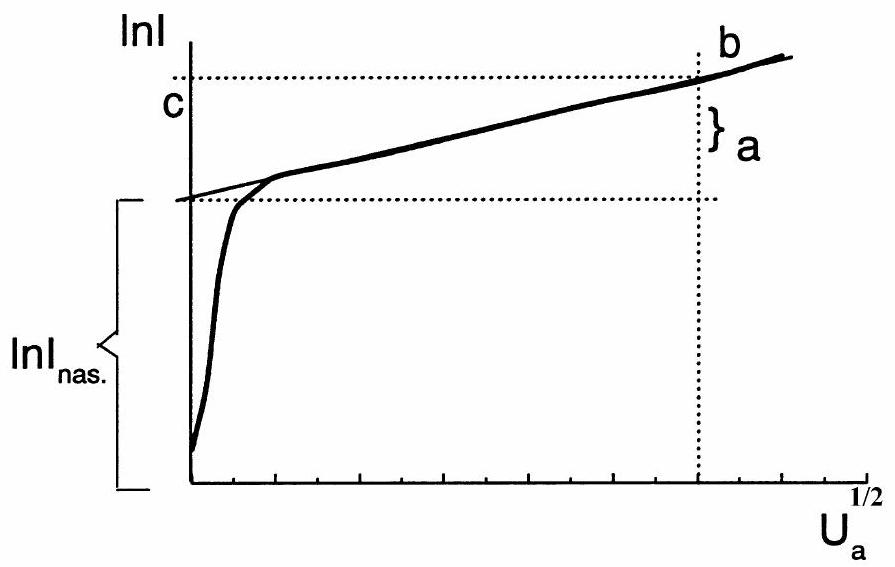
\includegraphics[width=0.7\linewidth]{primaumera}
			\caption{Závislost $I_{nas}$ na $U^{1/2}$, písm. $a$ značí přírustek proudu $\Delta I_{nas}$}
			\label{fig:primaumera}
		\end{figure}
		
		\subsection{Popis měřící aparatury}
		\begin{figure}[H]
			\centering
			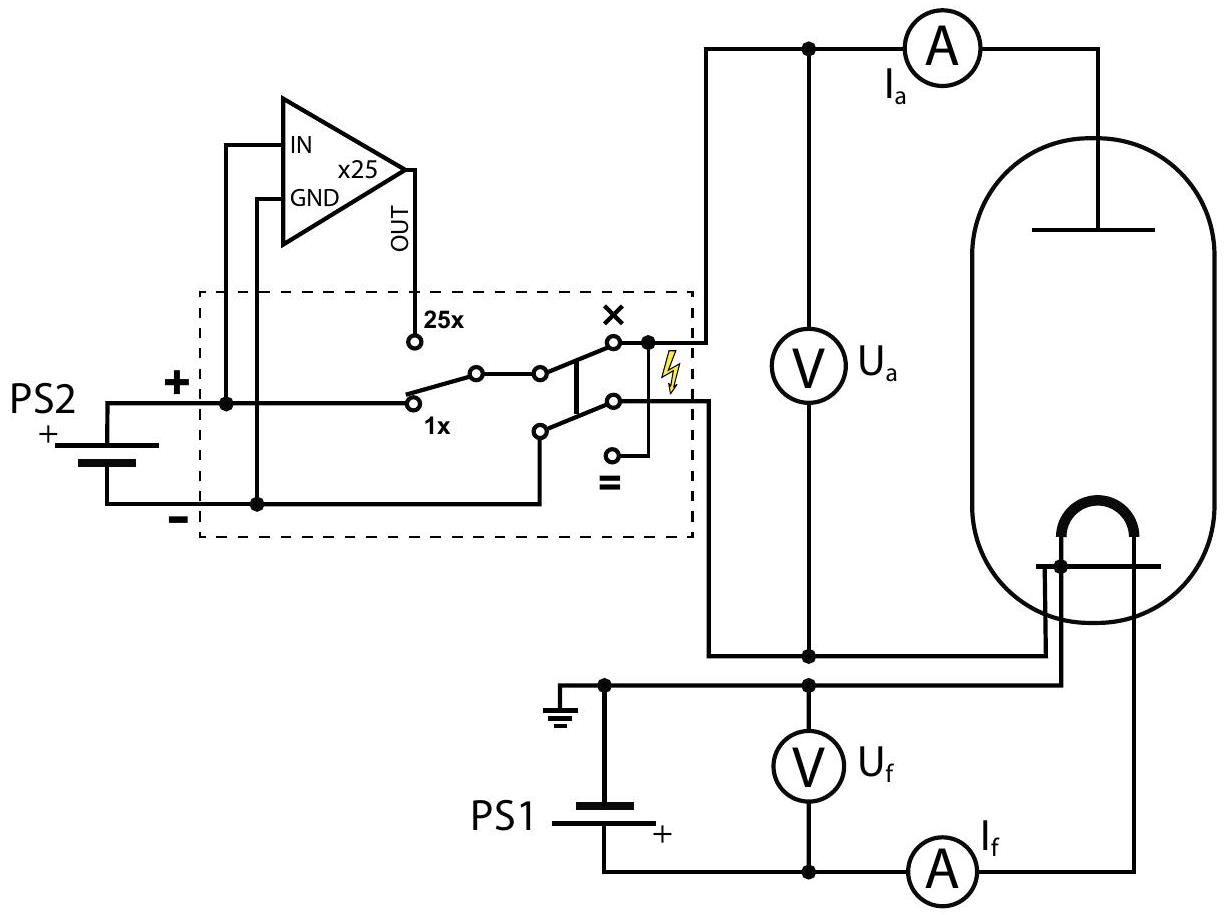
\includegraphics[width=0.7\linewidth]{zapojeni}
			\caption{Schéma zapojení experimentu}
			\label{fig:zapojeni}
		\end{figure}
		Aparaturu zapojujeme dle obr. 2; zdrojem PS2 s rozsahem 0-20V řídíme anodové napětí, přičemž napěťovým měničem v obvodu dokážeme napětí zvýšit 25krát pro realizaci napětí 500V. Druhý přepínač v obvodu zajišťuje změnu polarity bez nutnosti obvod rozpojovat. Druhý zdroj PS1 slouží ke žhavení wolframového vlákna.
		\newpage
		
		\section{Měření}
		Z Ohmova zákona získáme odpor vlákna pro žhavící proudy 1.92 a 1.98 A, úpravou formule (3) vypočteme teploty vlákna pro oba žhavící proudy. Získáváme:
		{\small \begin{align*}
			R_{192} & = 2.5432\pm2.10^{-4}\,\mathrm{\Omega} \quad T_{192}= 1173.27 \pm 0.11 \,\text{°C}\,\\
			R_{198} & = 2.5768\pm3.10^{-4 }\,\mathrm{\Omega} \quad T_{198}= 1192.47 \pm 0.15 \,\text{°C}
		\end{align*}}
		\subsection{VA charakteristika}
		Měříme VA charakteristiku anodového proudu na napětí. Při žhavícím proudu $1.92$ a $1.98$ A Zlogaritmované hodnoty proudu v náběhové části fitujeme lineárně, z formule (6) získáváme vztah mezi směrnicí a teplotou: $T = e/ka$.
		
		\begin{figure}[H]
		\centering
		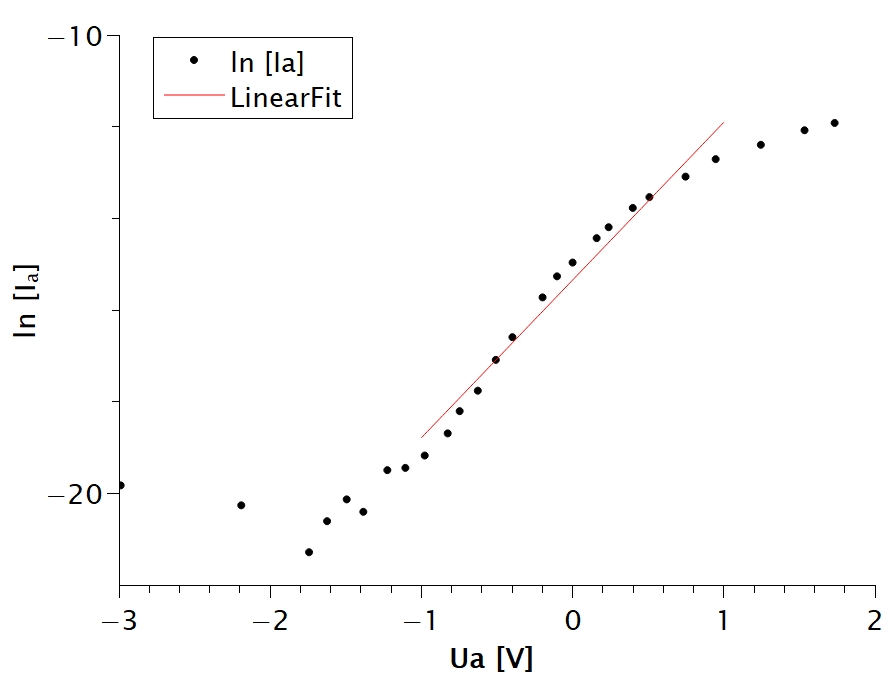
\includegraphics[width=0.7\linewidth]{192IaUa}
		\caption{Závislost $\ln I_a$ na $U_a$ pro žhavící napětí 1.92 A}
		\label{fig:192iaua - }
		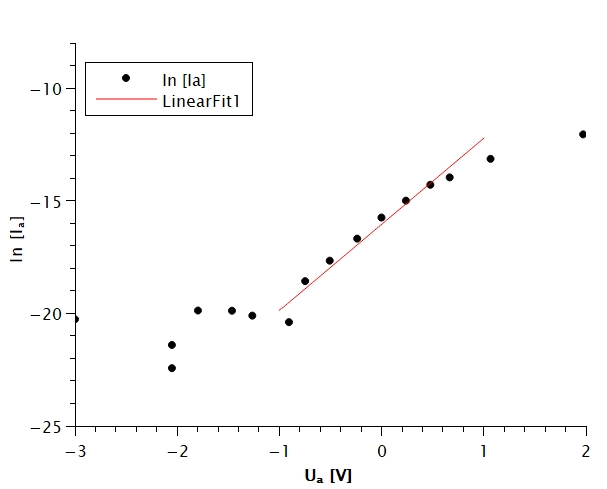
\includegraphics[width=0.7\linewidth]{198IaUa}
		\caption{Závislost $\ln I_a$ na $U_a$ pro žhavící napětí 1.98 A} 
		\end{figure}
		Ze směrnice lineárního proložení na obr. 3  a 4 pro hodnoty teploty získáváme		
		\begin{align*}
			T_{192} &= 3370 \pm 90 \,\text{K} \\
			T_{198}& = 3480 \pm 140 \,\text{K}.
		\end{align*}
		\quad \\
		\quad \\\quad \\
		\quad \\\quad \\
		
		\subsection{Schottkyho efekt}
		Vynesením závislosti $\ln I_a \propto \sqrt{U_a}$ a následným lineárním fitem (obr. 5,6) získáváme hodnoty $I_{nas}, \Delta I_{nas}$.
		\begin{figure}[H]
			\centering
			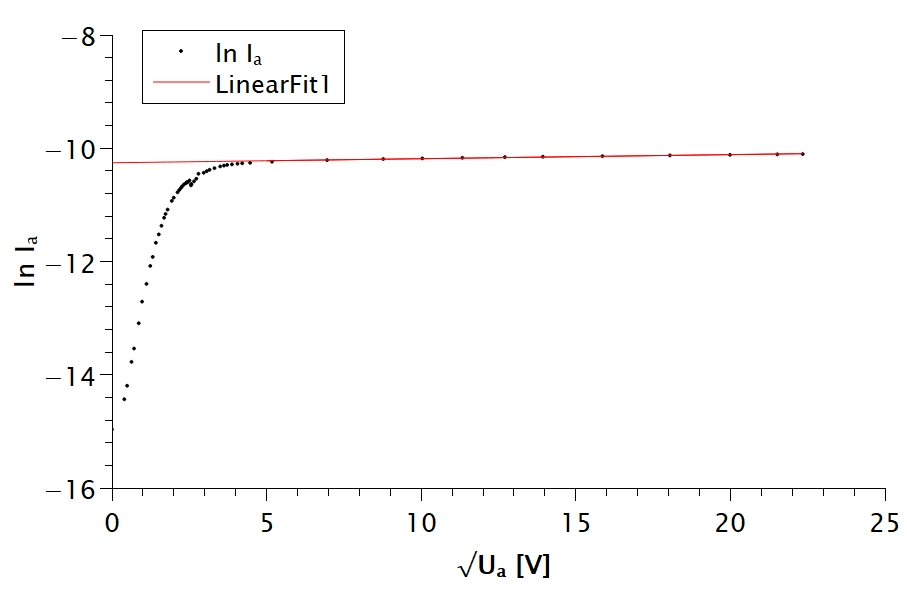
\includegraphics[width=0.7\linewidth]{192lnsq}
			\caption{Závislost $\ln I_a$ na $\sqrt{U_a}$ pro žhavící proud 1.92 A}
			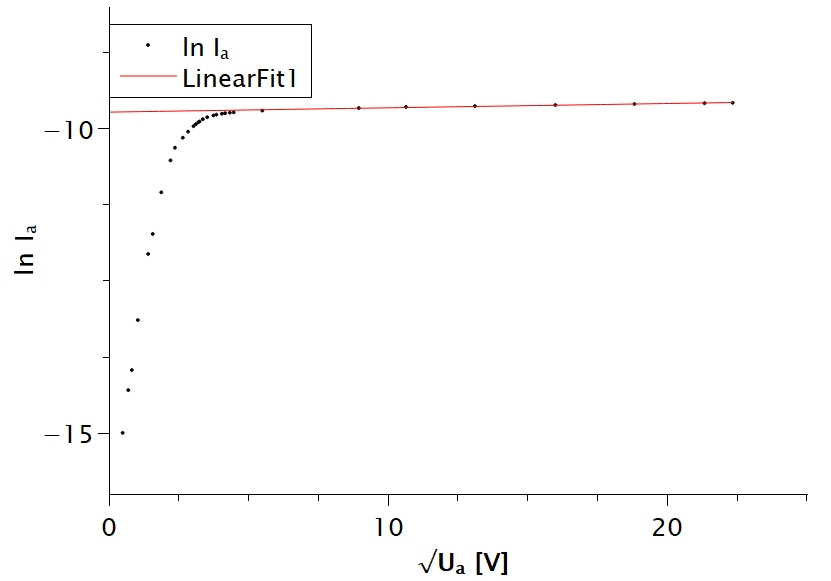
\includegraphics[width=0.7\linewidth]{198lnsq}
			\caption{Závislost $\ln I_a$ na $\sqrt{U_a}$ pro žhavící proud 1.98 A}
			\caption{b}
		\end{figure}\begin{align*}
			I_{nas192} &=  35.11 \pm 0.21 \,\mathrm{\mu A} \quad &\Delta I_{nas} =5.9 \pm 0.2 \,\mathrm{\mu A}\\
			I_{nas198} &=  59.7 \pm 0.5 \,\mathrm{\mu A}	\quad &\Delta I_{nas} = 9.8 \pm 0.5 \,\mathrm{\mu A}
		\end{align*}
		K nasycenému anodovému proudu dochází při napětích 19.95, resp. 21.4 V. Intenzita při $U_a = 500 \,\mathrm{V}$ je dle formule (13) $1.25\cdot10^6\,\rm Vm^{-1}$, teoretické hodnoty $\Delta I_{nas}$ jsou
		\begin{align*}
		&\Delta I_{nas} =24.99 \pm 0.15 \,\mathrm{\mu A}\\
		&\Delta I_{nas} = 42.6 \pm 0.3 \,\mathrm{\mu A}
		\end{align*} \newpage
		\subsection{Výstupní práce}
		Ze závislosti změřeného anodového proudu na žhavícím proudu vykreslíme závislost $\ln \frac{I_{nas}}{T^2}, f(1/T)$:
			\begin{figure}[H]
			\centering
			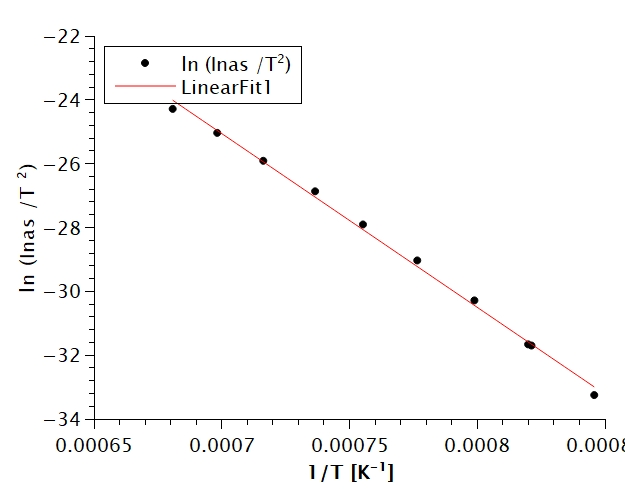
\includegraphics[width=0.7\linewidth]{vystupniprace}
		\end{figure}
		Získáváme hodnoty:
		\begin{align*}
			& w = 4.69 \pm 0.09 \,\mathrm{eV}\\
		\end{align*}
		\section{Závěr}
		Pro všechna měření se nám podařilo získat výsledky. V případě výstupní práce je výsledek smysluplné, od skutečné výstupní práce se značně neodchyluje. Při srovnání teoretických a měřených hodnot $\Delta I_{nas}$ již pozorujeme větší rozdíly. \\ Získaná hodnota teploty elektronů má význam spíše jen orientační - neočekáváme od ni velikou přesnost, jelikož určení hranice náběhové oblasti pro provedení lineární aproximace nebylo jednoznačné. Lze nicméně pozorovat, že je teplota elektronů u vyššího žhavícího proudu též vyšší.
	
		

		
		
		
		
		
		% Nakonec nezapomeňte projet text programem vlna nebo vlnka, např.
		% 	vlna -m -l -n mojeuloha.tex
		% nebo zkontrolovat a opravit jednopísmenné předložky na koncích řádků ručně.
	\end{multicols}
\end{document}
